\documentclass[professionalfont]{beamer}

\usepackage{graphicx}
\usepackage{newtxtext,newtxmath}
\usetheme{default}
\usecolortheme{seagull}

\setbeamertemplate{navigation symbols}{}
\setbeamertemplate{itemize item}{\textbullet} 
\setbeamertemplate{title page}{
    \begin{center}
        {\textcolor{blue}{\textbf{\fontsize{11}{14}\selectfont OlympiadBench: A Challenging Benchmark for Promoting AGI with Olympiad-Level Bilingual Multimodal Scientific Problems}}} \\[1.5cm]
        
        {\fontsize{9}{14}\selectfont Chaoqun He, et al \\[0.3cm]
        Tsinghua University \\[0.3cm]
        June 6, 2024}
    \end{center}
}
% ------------------ Title ------------------

\begin{document}
\frame{\titlepage}


\begin{frame}
\begin{center}
    { \textbf{\textcolor{blue}{ {\fontsize{12}{14}\selectfont Abstract} }} }
\end{center}
\\[0.5cm]

{\fontsize{10}{14}\selectfont 
\begin{itemize}
    \item This benchmark consists of problems from exam, competitions
    \item Each problem is detailed with expert-level annotations
    \item Even GPT-4V attained an average score of 17.97\%
\end{itemize}
}

\end{frame}
% ------------------ Slide 1 ------------------

\begin{frame}
\begin{center}
    { \textbf{\textcolor{blue}{ {\fontsize{12}{14}\selectfont Introduction} }} }
\end{center}
\\[0.2cm]

\begin{center}
    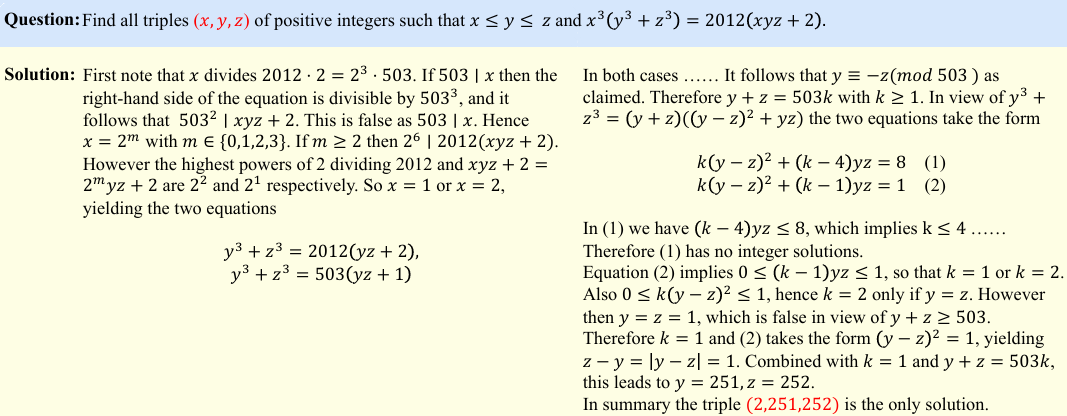
\includegraphics[width=1.0\textwidth]{figure1.png}
\end{center}

{\fontsize{10}{14}\selectfont 
\begin{itemize}
    \item Many benchmarks lack sufficient challenge for the latest models
    
    - GPT-4 with prompting techniques has achieved 97.0\% on GSM8K
    
    - They focus on text, unable to understand geometry and physics
\end{itemize}
}

\end{frame}
% ------------------ Slide 2 ------------------

\begin{frame}
\begin{center}
    { \textbf{\textcolor{blue}{ {\fontsize{12}{14}\selectfont Dataset} }} }
\end{center}
\\[0.2cm]

\begin{center}
    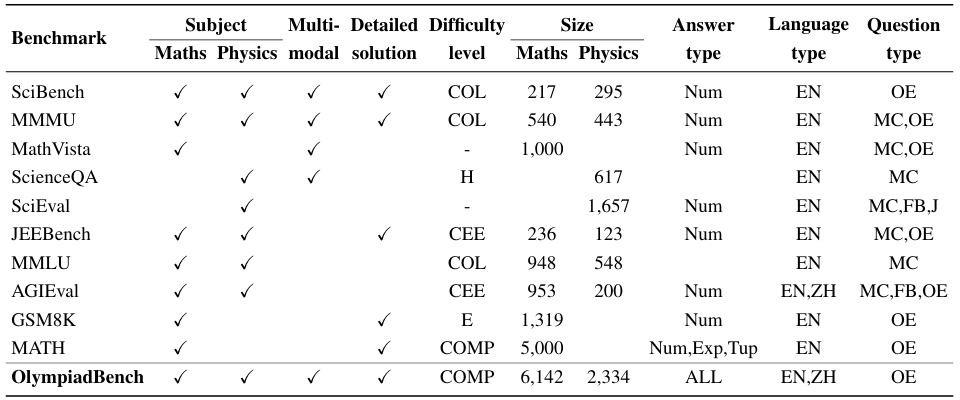
\includegraphics[width=1.0\textwidth]{table1.png}
\end{center}

{\fontsize{9}{14}\selectfont 
\begin{itemize}
    \item Difficulty level (COMP, COL, CEE, H, E)
    
    - Competition, College, College Entrance Exam, High / Elementary School

    \item Bilingual
    
    - EN for English, ZH for Chinese
\end{itemize}
}

\end{frame}
% ------------------ Slide 3 ------------------

\begin{frame}
\begin{center}
    { \textbf{\textcolor{blue}{ {\fontsize{12}{14}\selectfont Experiment} }} }
\end{center}
\\[0.2cm]

\begin{center}
    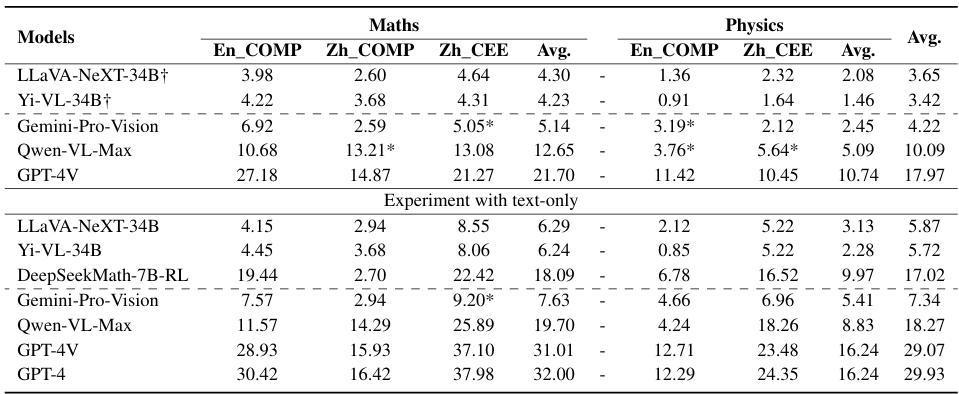
\includegraphics[width=1.0\textwidth]{table4.png}
\end{center}

{\fontsize{10}{14}\selectfont 
\begin{itemize}
    \item Performance drop in physics, Chinese, image problems
\end{itemize}
}

\end{frame}
% ------------------ Slide 4 ------------------

\begin{frame}
\begin{center}
    { \textbf{\textcolor{blue}{ {\fontsize{12}{14}\selectfont Experiment} }} }
\end{center}
\\[0.2cm]

\begin{center}
    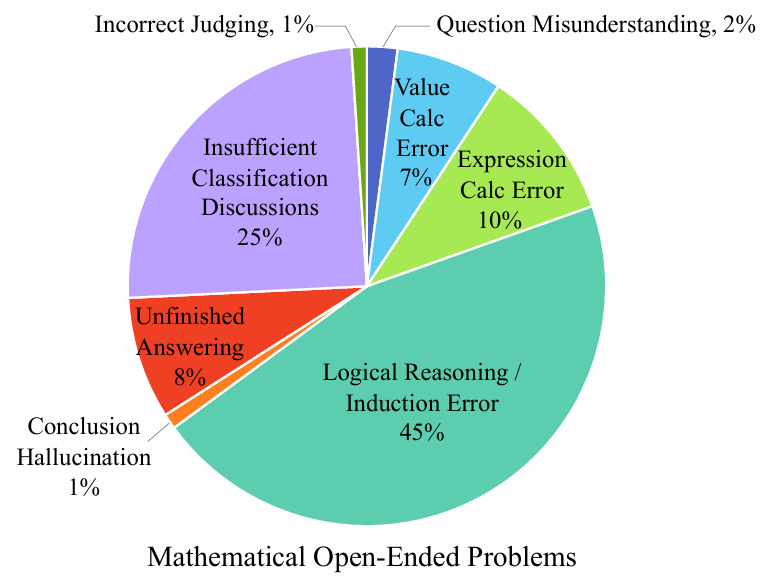
\includegraphics[width=0.6\textwidth]{figure4-1.png}
\end{center}

{\fontsize{10}{14}\selectfont 
\begin{itemize}
    \item Mathematics Error

    - Logical Reasoning Error(45\%)
    
    - Insufficient classification in Combinatorial problems(25\%)
    
    - Large Calculation Error(10\%)
    
\end{itemize}
}

\end{frame}
% ------------------ Slide 5 ------------------

\begin{frame}
\begin{center}
    { \textbf{\textcolor{blue}{ {\fontsize{12}{14}\selectfont Experiment} }} }
\end{center}
\\[0.2cm]

\begin{center}
    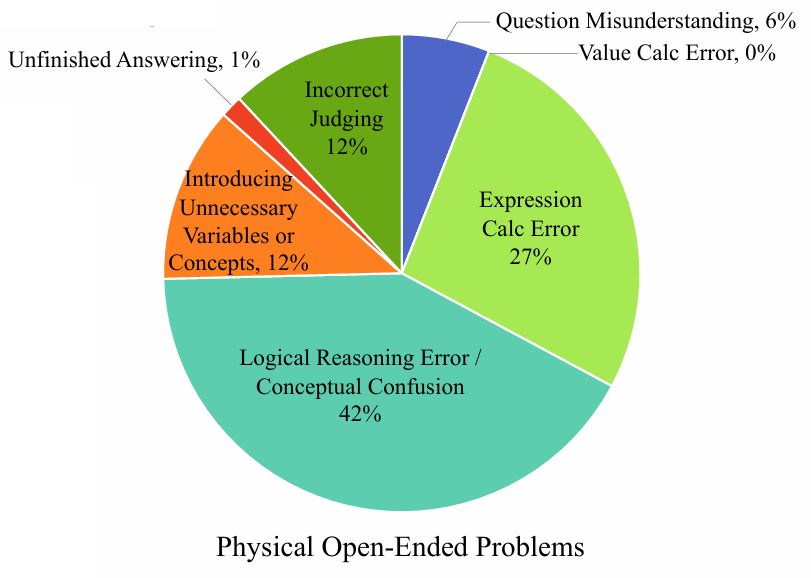
\includegraphics[width=0.6\textwidth]{figure4-2.png}
\end{center}

{\fontsize{10}{14}\selectfont 
\begin{itemize}
    \item Physics Error

    - Logical Reasoning Error(42\%) 
    
    - Large Calculation Error(25\%)
    
    - Introducing unnecessary variables(12\%)
    
\end{itemize}
}

\end{frame}
% ------------------ Slide 6 ------------------

\begin{frame}
\begin{center}
    { \textbf{\textcolor{blue}{ {\fontsize{12}{14}\selectfont Conclusion} }} }
\end{center}
\\[0.2cm]

{\fontsize{10}{14}\selectfont 
\begin{itemize}
    \item We proposed advanced benchmark

    - Each problem is detailed with expert-level annotations
    
    - Pinpointing prevalent error types

    \item Limitations

    - There are proof problems

    - Code generation or automated verification is impossible
\end{itemize}
}

\end{frame}
% ------------------ Slide 7 ------------------


\end{document}
